\section{Различные улучшения алгоритма Position Based Dynamics} \label{ch2:pbd-improvments} %название по-русски
	Алгоритм, описанный в предыдущей главе, позволяет симулировать поведение мягких тел, однако не может быть применен на практике из-за отсутствия обработки взаимодействия с другими симулируемыми телами, а также большим временным затратам. В связи с этим, в статье \cite{pbd}, помимо основной идеи алгоритма, были предложены различные улучшения.
	
	Во-первых, требуется исправить то, что симулируемое описанным образом мягкое тело не взаимодействует с другими физическими телами. Это означает, что при визуализации симулируемого тела можно будет наблюдать, \say{прохождение сквозь} другие тела. Для недопущения таких ситуаций, используются алгоритмы обнаружения и обработки столкновений. В статье \cite{pbd} для решения этой проблемы предлагается динамически создавать новые ограничения с параметрами:
	\begin{enumerate}[1.]
		\item Функция $C(p) = (p - q) * n$, где $q$ - точка пересечения луча, выходящего из положения частицы $p$ в направлении предсказанного положения частицы $p^*$, с поверхностью твердого объекта, а $n$ - вектор нормали к поверхности данного объекта в точке $q$.
		\item Параметр жесткости $k = 1$.
		\item Тип ограничения \say{неравенство}.
	\end{enumerate}
	
	Таким образом получается достичь \say{одностороннего взаимодействия} - мягкое тело отткалкивается от твердых, но твердые тела не изменяют свои импульсы в результате столкновений с мягкими. Чтобы добиться \say{двухстороннего взаимодействия}, авторами было принято решение придавать твёрдому телу импульс, равный $\frac{m_i*(p_i(t + \Delta t) - p_i(t))}{\Delta t}$ за каждую частицу, для которой было обнаружено пересечение.
		
	Во-вторых, необходимо исправить такую проблему: симулирумое мягкое тело не взаимодействует с частями самого себя. То есть если частицы не соединены ограничениями напрямую, то эти частицы могут свободно перемещаться друг относительно друга, что визуально приводит к самопересечениям. В статье \cite{pbd} авторы предлагают разбить поверхность мягкого тела на треугольники и проверять пересечение частиц, с треугольниками заданными тремя вершинами $p_1^t, p_2^t, p_3^t$ и толщиной $h$, при помощи функций:
	\begin{equation}
		C(p^*, p_1^t, p_2^t, p_3^t) = (p^* - p_1^t) \cdot \frac{(p_2^t - p_1^t) \times (p_3^t - p_1^t)}{|(p_2^t - p_1^t) \times (p_3^t - p_1^t)|} - h
	\end{equation}
	
	Или, если частица входит в треугольник со стороны обратной стороне нормали:
	\begin{equation}
		C(p^*, p_1^t, p_2^t, p_3^t) = (p^* - p_1^t) \cdot \frac{(p_3^t - p_1^t) \times (p_2^t - p_1^t)}{|(p_3^t - p_1^t) \times (p_2^t - p_1^t)|} - h
	\end{equation}	
	
	Таким образом возможно избавиться от самопересечений, однако, если просто проверять все возможные частицы со всеми возможными треугольниками, данный алгоритм окажется излише нагруженным с точки зрения времени выполнения. Для того, чтобы убрать из рассмотрения часть проверяемых треугольников, авторами используется алгоритм пространственного хеширования треугольников, описанный в \cite{teschner2003optimized}.
	
	В-третьих, для удаления излишних колебаний, авторы используют демпфирование, уменьшая скорости, полученные на этапе предсказания положений частиц, используя константу демпфирования. 
	
	Применив вышеописанные улучшения, достигается возможность симулировать поверхность ткани, разрываемой в результате взаимодействия с физическими объектами, как показано на \firef{fig:tearcloth}. Результирующий алгоритм представлен на \firef{alg:PositionBasedDynamics2}.
	
	\begin{figure}[ht!] 
		\center
		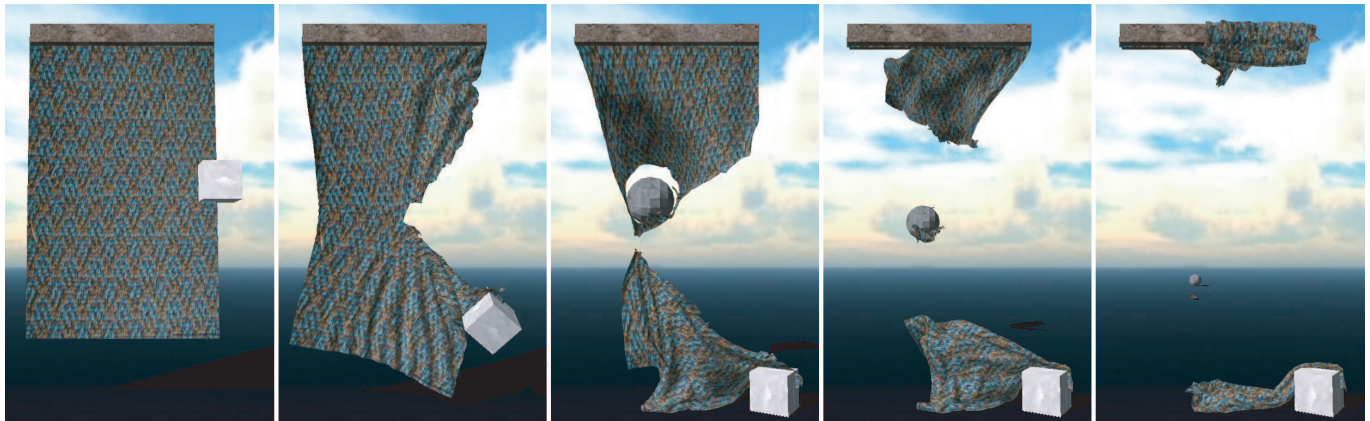
\includegraphics [scale=0.3] {my_folder/images//tear_cloth}
		\caption{Пример куска ткани, разорванного в следствии взаимодействия с летящей сферой и закрепленным кубом.}
		\label{fig:tearcloth}  
	\end{figure}
	
	\begin{algorithm} %[h]
		\SetKwFunction{algoPBDTwoPseudocode}{} 
		\SetKwProg{myalg}{Algorithm}{}{} %write in 2nd agrument <<Algorithm>>, <<Procedure>> etc
		\nonl\myalg{\algoPBDTwoPseudocode}{
			\KwInput{
				время шага симуляции $\Delta t$,
				количество итераций $solverIteration$,
				текущее и предыдущее состояние частиц,
				ограничения,
				функция внешних сил от положения $f_{ext}(p)$,
			}
			\KwOutput{положение частиц спустя заданное время $\{p_i(t + \Delta t)\}_N$}
			
			\lFor {$i \in 1..N $\label{step:pbd2-solver-integrate-vel}}{
				$v_i = \frac{p_i(t) - p_i(t -\Delta t)}{\Delta t} + \Delta t * im_i * f_{ext}(p_i)$
			}
			
			$dampVelocities(v_1, ... v_N)$;
			
			\lFor {$i \in 1..N$\label{step:pbd2-solver-integrate-pos}}{
				$p^*_i = p_i(t) + v_i * \Delta t $
			}

			\lFor {$i \in 1..N $\label{step:pbd2-solver-collision}}{
				$genCollisionConstraints(p_i -> p^*_i)$;
			}
			
			\For{$k \in 1..solverIteration$  \label{step:pbd2-solver-loop}}{
				$p^*_1, ..., p^*_N = projectConstraints(p^*_1, ..., p^*_N)$;
			}
			
			\lFor {$i \in 1..N $\label{step:pbd2-solver-save}}{
				$p_i(t + \Delta t) = p^*_i$\
			}
		}
		\caption{Псевдокод алгоритма Position Based Dynamics с учетом коллизий и демпфирования}\label{alg:PositionBasedDynamics2}
	\end{algorithm}
	\FloatBarrier
	
	Как можно заметить, временная сложность данного алгоритма пропорциональна произведению числа частиц на число итераций. В связи с этим, авторы многих статей ставили перед собой цель уменьшить два этих параметра, при этом сохраняя точность.
	
	Так, в статье \cite{muller2010wrinkle} авторами было замечено, что при увеличении размерности сетки, основным визуальным улучшением являются небольшие складки, не сильно влияющие на глобальное поведение ткани. Тогда было решено разделить ткань на глобальную сетку с низким числом частиц и локальную сетку с высоким числом частиц. Основной алгоритм симуляции ткани (вместе с обработкой пересечений) применялся к глобальной сетке. Локальная сетка же, прикреплялась к глобальной сетке, и её симуляция не требовала большого количества итераций (\firef{fig:wrincle-idea} и \firef{fig:wrincle-show}).

	\begin{figure}[ht!] 
		\center
		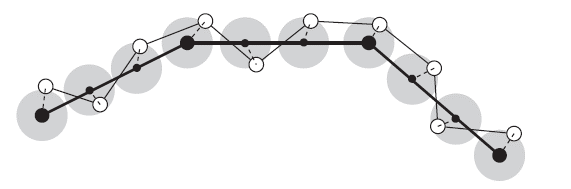
\includegraphics [scale=0.7] {my_folder/images//wrincle_mesh_idea}
		\caption{Схема, поясняющая идею алгоритма складок. Черные точки - вершины глобальной сетки, белые точки - вершины локальной сетки. Прикрепление локальной сетки к глобальной происходит за счет добавления ограничений на расстояние, представленых в виде серых дисков}
		\label{fig:wrincle-idea}  
	\end{figure}
	
		
	\begin{figure}[ht!] 
		\center
		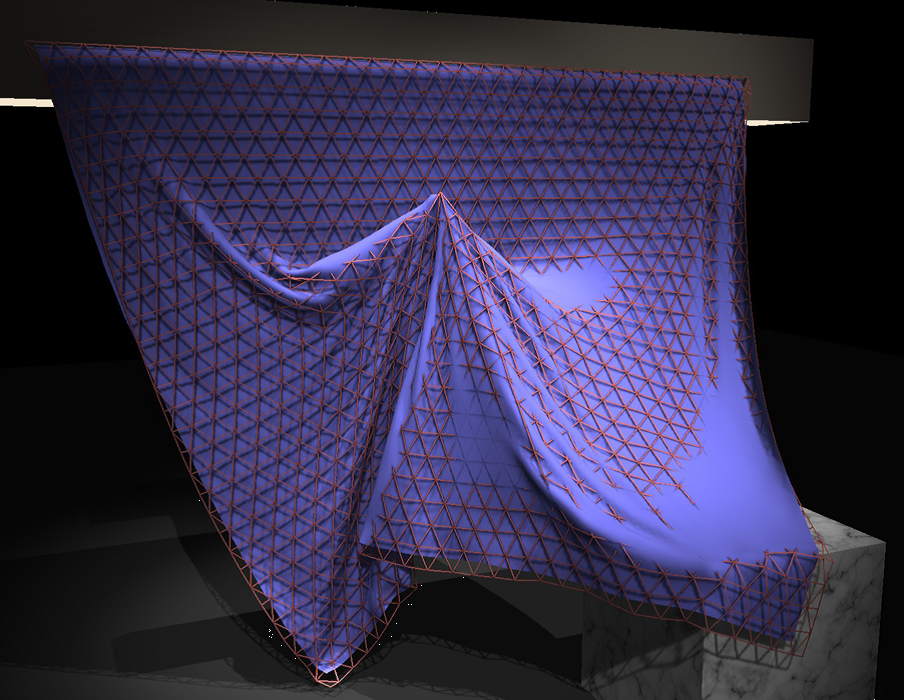
\includegraphics [scale=0.5] {my_folder/images//wrincle_mesh_show}
		\caption{Визуальная демонстрация алгоритма складок. Красным представлена глобальная сетка, а фиолетоым представлена ткань локальной сетки}
		\label{fig:wrincle-show}  
	\end{figure}
	
	А в другой статье \cite{kim2012long} авторами была предпринята попытка решить проблему глобального растяжения ткани в случае малого числа итераций. Для этого они разработали технику Long Range Attachments (LRA). Она основывается на том, что зачастую растяжение ткани проявляется в ситуациях, когда какие-либо частицы ткани закреплены в пространстве. Идея данной техники заключается в том, чтобы связывать ограничениями не только соседние вершины. Добавив дополнительные ограничения, связывающие закрепленные вершины с другими вершинами (как показано на \firef{fig:lra}) можно ограничить смещения незакрепленных частиц относительно закрепленных, тем самым избавляясь от излишнего растяжения.
	
	\begin{figure}[ht!] 
		\center
		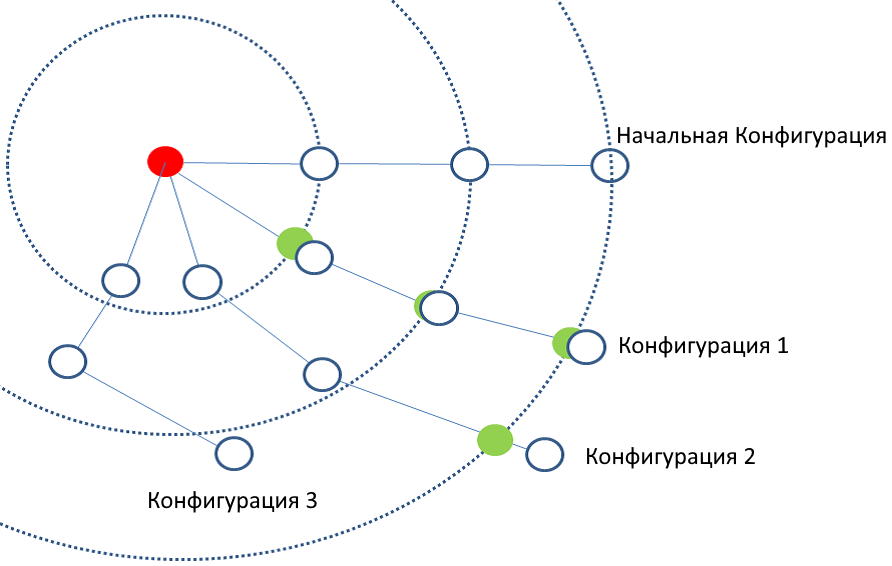
\includegraphics [scale=0.53] {my_folder/images//lra}
		\caption{Схема, поясняющая идею алгоритма Long Range Attachments на примере нерастяжимой веревки. Красным цветом обозначена закрепленная вершина. Каждая другая вершина удерживается или остается внутри соответствующей ей сферы (представленной пунктиром). Для каждой конфигурации (если вершина оказалась за пределами своей сферы) зеленым представлено положение, исправленное алгоритмом LRA}
		\label{fig:lra}  
	\end{figure}
	
%% Вспомогательные команды - Additional commands
%
%\newpage % принудительное начало с новой страницы, использовать только в конце раздела
%\clearpage % осуществляется пакетом <<placeins>> в пределах секций
%\newpage\leavevmode\thispagestyle{empty}\newpage % 100 % начало новой страницы